\documentclass[10pt,aspectratio=169]{beamer}

%================================================
% Theme
%================================================
\usetheme[numbering=fraction,progressbar=frametitle]{metropolis}
\metroset{sectionpage=none}

%================================================
% Packages
%================================================
\usepackage{amsmath,amssymb}
\usepackage{booktabs}
\usepackage{tikz}
\usetikzlibrary{automata,positioning,arrows.meta,calc,shapes.geometric}
\usepackage{xcolor}
\usepackage{listings}

%================================================
% Metadata
%================================================
\newcommand{\LastCompiled}{\today}

\title{Theory of Computation}
\subtitle{Lecture 6: Non-Regular Languages\\The Pumping Lemma}
\author{Sheikh Azizul Hakim\\Lecturer, Department of CSE, BUET}
\date{Last compiled: \LastCompiled}

%================================================
% Listings
%================================================
\lstdefinestyle{code}{
  basicstyle=\ttfamily\small,
  frame=single,
  backgroundcolor=\color{black!4},
  rulecolor=\color{black!20},
  showstringspaces=false,
  columns=fullflexible,
  keepspaces=true
}
\lstset{style=code}

%================================================
% Helpers
%================================================
\newcommand{\eps}{\varepsilon}
\newcommand{\lang}[1]{\mathsf{#1}}
\newcommand{\N}{\mathbb N}

\tikzset{
  every state/.style={minimum size=8mm},
  >=Stealth,
  shorten >=1pt,
}

%================================================
\begin{document}

\maketitle

%------------------------------------------------
\begin{frame}[standout]
Finite automata are powerful.

But finite memory has fundamental mathematical limits.
\end{frame}

%------------------------------------------------
\begin{frame}{Today's Roadmap}
\begin{enumerate}
    \item \textbf{The Graph Intuition:} Why finite states force repetition.
    \item \textbf{The Formal Theorem:} Sipser's Pumping Lemma.
    \item \textbf{The Adversary Game:} How to navigate the nested quantifiers.
    \item \textbf{The Proof Template:} A rigorous, step-by-step recipe for contradictions.
    \item \textbf{Worked Examples:} Proving languages are non-regular.
\end{enumerate}
\end{frame}

%================================================
\section{1. The Graph Intuition: Finite States, Infinite Strings}

%------------------------------------------------
\begin{frame}{A Suspicious Language}

Consider the language of perfectly balanced binary strings:
\[
B = \{0^n1^n \mid n \geq 0\}
\]

\vspace{0.8em}
To accept $00001111$, a machine must somehow ``remember'' that it saw exactly four $0$s so it can verify the four $1$s.

\vspace{0.8em}
\textbf{The problem:} A DFA only has a fixed number of states (say, $p$ states). What happens when we feed it $p+1$ zeros?

\end{frame}

%------------------------------------------------
\begin{frame}{The Pigeonhole Principle in Directed Graphs}

A DFA is simply a directed graph. 
Reading a string is just tracing a walk through that graph.

\vspace{0.8em}
\textbf{Pigeonhole Principle:} If you put $m+1$ pigeons into $m$ holes, at least one hole contains two pigeons.

\vspace{0.8em}
If a DFA has $p$ states, and it reads a string of length $p$ or greater, it visits at least $p+1$ states (counting the start state).
Therefore, \textbf{it must visit at least one state twice.}

\end{frame}

%------------------------------------------------
\begin{frame}{Revisiting a State Creates a Cycle}

In graph theory, a walk that intersects itself contains a cycle. 

\vspace{0.8em}
Let the string be $s = xyz$.
\begin{itemize}
    \item $x$: The path from the start state to the first time we hit the repeated state.
    \item $y$: The cycle (leaving the state and returning to it).
    \item $z$: The path from the repeated state to the accept state.
\end{itemize}

\begin{center}
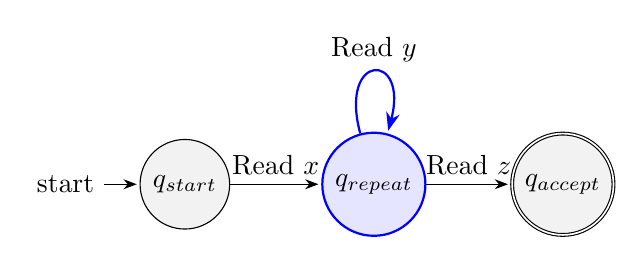
\begin{tikzpicture}[
  ->,>=Stealth,shorten >=1pt,
  node distance=2.4cm,
  every state/.style={minimum size=8mm, fill=black!5}
]
  \node[state, initial] (q0) {$q_{start}$};
  \node[state, fill=blue!10, draw=blue, thick, right of=q0] (q) {$q_{repeat}$};
  \node[state, accepting, right of=q] (f) {$q_{accept}$};
  \path
    (q0) edge node[above] {Read $x$} (q)
    (q) edge[loop above, thick, blue] node[black] {Read $y$} ()
    (q) edge node[above] {Read $z$} (f);
\end{tikzpicture}
\end{center}

\end{frame}

%------------------------------------------------
\begin{frame}{The ``Pump''}

Because $y$ is a cycle, the DFA doesn't actually know how many times it loops. 
If the DFA accepts $xyz$, it has no choice but to also accept:

\vspace{0.5em}
\begin{itemize}
    \item $xz$ (looping 0 times, skipping $y$)
    \item $xyyz$ (looping 2 times)
    \item $xyyyz$ (looping 3 times)
\end{itemize}

\vspace{0.8em}
\textbf{Core Intuition:} Any sufficiently long string accepted by a regular language MUST contain a cycle that can be ``pumped'' (repeated) infinitely without leaving the language.

\end{frame}

%================================================
\section{2. The Formal Theorem}

%------------------------------------------------
\begin{frame}{The Pumping Lemma for Regular Languages}

\begin{block}{}
If $A$ is a regular language, then there exists a number $p$ (the pumping length) such that every string $s \in A$ with $|s| \geq p$ can be divided into three pieces, $s = xyz$, satisfying the following three conditions:
\vspace{0.5em}
\begin{enumerate}
    \item for each $i \geq 0$, $xy^iz \in A$,
    \item $|y| > 0$, and
    \item $|xy| \leq p$.
\end{enumerate}
\end{block}

\vspace{0.8em}
\textit{Why $|y| > 0$?} The cycle must consume at least one character, or we aren't pumping anything. \\
\textit{Why $|xy| \leq p$?} By the Pigeonhole Principle, the first duplicate state MUST occur within the first $p$ steps. 

\end{frame}

%================================================
\section{3. The Adversary Game (Quantifier Logic)}

%------------------------------------------------
\begin{frame}{The Logic of Contradiction}

The Pumping Lemma is an implication: 
\[ \text{IF } A \text{ is regular} \implies A \text{ has the pumping property.} \]

\vspace{0.8em}
By modus tollens, if $A$ does \textbf{not} have the pumping property, it is \textbf{not} regular.

\vspace{0.8em}
The lemma relies on heavily nested quantifiers:
\[ \exists p, \forall s, \exists x,y,z, \forall i \dots \]

To prove a language is NOT regular, we must negate this statement:
\[ \forall p, \exists s, \forall x,y,z, \exists i \dots \]

\end{frame}

%------------------------------------------------
\begin{frame}{How to play The Adversary Game}

Think of the proof as a turn-based game against the SETUP DEMON who claims $A$ is regular. You win if you force a contradiction.

\vspace{0.8em}
\begin{table}
\centering
\begin{tabular}{lp{8cm}}
\toprule
\textbf{Turn} & \textbf{Action} \\
\midrule
\textbf{1. Demon:} & Chooses the pumping length $p$. (You don't know $p$, it's a variable). \\
\textbf{2. YOU:} & Choose a target string $s \in A$ such that $|s| \geq p$. \\
\textbf{3. Demon:} & Divides your string into $s = xyz$ however they want, as long as $|y|>0$ and $|xy| \le p$. \\
\textbf{4. YOU:} & Choose a pump count $i \ge 0$ such that $xy^iz \notin A$. \\
\bottomrule
\end{tabular}
\end{table}

\vspace{0.8em}
\textbf{Rule of Rigor:} You cannot choose the split ($x,y,z$). You must prove your $i$ works for \textit{any} valid split the Demon could possibly make.

\end{frame}

%================================================
\section{4. The Proof Template}

%------------------------------------------------
\begin{frame}{The Rigorous 5-Step Proof Template}

Every valid Pumping Lemma proof follows exactly this structure. \textbf{Do not skip steps.}

\vspace{0.5em}
\begin{enumerate}
    \item \textbf{Assume for contradiction} that language $L$ is regular.
    \item Let $p$ be the pumping length given by the Pumping Lemma.
    \item \textbf{Choose a specific string} $s \in L$ where $|s| \geq p$. \\
          \textit{(This is your creative step. Express $s$ in terms of $p$.)}
    \item State that by the lemma, $s$ can be split into $s = xyz$ such that $|y|>0$ and $|xy| \le p$. \textbf{Analyze what $y$ must look like} based on the $|xy| \le p$ constraint.
    \item \textbf{Pump} the string. Choose an $i \ge 0$. Show mathematically that $xy^iz \notin L$, creating a contradiction. Conclude $L$ is not regular.
\end{enumerate}

\end{frame}


%================================================
\section{5. Worked Examples}

%------------------------------------------------
\begin{frame}{Example 1: Matching Two Blocks}

\small
\[
L_1=\{0^n1^n\mid n\geq 0\}.
\]

\begin{enumerate}
    \item \textbf{Assume for contradiction} that $L_1$ is regular.
    \item Let $p$ be its pumping length.
    \item Choose
    \[
    s=0^p1^p.
    \]
    Clearly, $s\in L_1$ and $|s|=2p\geq p$.
    \item For every valid split $s=xyz$ with $|xy|\leq p$ and $|y|>0$, both $x$ and $y$ lie inside the first block of $0$s. Hence
    \[
    y=0^k\qquad\text{for some }1\leq k\leq p.
    \]
\end{enumerate}

\end{frame}

%------------------------------------------------
\begin{frame}{Example 1: Pumping Breaks Equality}

\small
\begin{enumerate}
    \setcounter{enumi}{4}
    \item Choose $i=0$. Then
    \[
    xy^0z=xz=0^{p-k}1^p.
    \]
    The pumped string contains $p-k$ zeros but still contains $p$ ones.

    Since $k>0$,
    \[
    p-k\neq p.
    \]
    Therefore,
    \[
    xz\notin L_1.
    \]
\end{enumerate}

This contradicts the Pumping Lemma. Therefore, $L_1$ is not regular.
\hfill $\blacksquare$

\vspace{0.7em}
\begin{block}{Intuition}
The machine is forced to repeat or remove some early $0$s without changing the later $1$s.
\end{block}

\end{frame}

%------------------------------------------------
\begin{frame}{Example 2: Palindromes}

\small
\[
L_2=\{w\in\{a,b\}^*\mid w=w^R\}.
\]

\begin{enumerate}
    \item \textbf{Assume for contradiction} that $L_2$ is regular.
    \item Let $p$ be its pumping length.
    \item Choose
    \[
    s=a^pba^p.
    \]
    This string is a palindrome and $|s|=2p+1\geq p$.
    \item For every valid split $s=xyz$, the condition $|xy|\leq p$ forces $y$ to lie entirely inside the first block of $a$s. Thus,
    \[
    y=a^k\qquad\text{for some }1\leq k\leq p.
    \]
\end{enumerate}

\end{frame}

%------------------------------------------------
\begin{frame}{Example 2: Pumping Breaks Symmetry}

\small
\begin{enumerate}
    \setcounter{enumi}{4}
    \item Choose $i=0$. Then
    \[
    xy^0z=a^{p-k}ba^p.
    \]
    The left side of the central $b$ has $p-k$ copies of $a$, while the right side has $p$ copies.

    Because $k>0$, the two sides are unequal. Hence the string is not a palindrome:
    \[
    xy^0z\notin L_2.
    \]
\end{enumerate}

This contradicts the Pumping Lemma. Therefore, $L_2$ is not regular.
\hfill $\blacksquare$

\vspace{0.7em}
\begin{block}{Intuition}
Pumping changes only the left half, so the mirror image no longer matches.
\end{block}

\end{frame}

%------------------------------------------------
\begin{frame}{Example 3: Synchronizing Three Blocks}

\small
\[
L_3=\{a^nb^nc^n\mid n\geq 0\}.
\]

\begin{enumerate}
    \item \textbf{Assume for contradiction} that $L_3$ is regular.
    \item Let $p$ be its pumping length.
    \item Choose
    \[
    s=a^pb^pc^p.
    \]
    Clearly, $s\in L_3$ and $|s|=3p\geq p$.
    \item For every valid split $s=xyz$, $|xy|\leq p$ places $y$ completely inside the initial block of $a$s. Therefore,
    \[
    y=a^k\qquad\text{for some }1\leq k\leq p.
    \]
\end{enumerate}

\end{frame}

%------------------------------------------------
\begin{frame}{Example 3: One Block Changes, Two Do Not}

\small
\begin{enumerate}
    \setcounter{enumi}{4}
    \item Choose $i=2$. Then
    \[
    xy^2z=a^{p+k}b^pc^p.
    \]
    The numbers of $a$s, $b$s, and $c$s are now
    \[
    p+k,\quad p,\quad p.
    \]
    Since $k>0$, these three quantities are not equal. Thus,
    \[
    xy^2z\notin L_3.
    \]
\end{enumerate}

This contradicts the Pumping Lemma. Therefore, $L_3$ is not regular.
\hfill $\blacksquare$

\vspace{0.7em}
\begin{block}{Intuition}
A finite automaton cannot keep three arbitrarily large blocks perfectly synchronized.
\end{block}

\end{frame}

%------------------------------------------------
\begin{frame}{Example 4: Copying Across a Separator}

\small
\[
\Sigma = \{0, 1, \#\} \qquad 
L_4=\{w\#w\mid w\in\{0,1\}^*\}.
\]

\begin{enumerate}
    \item \textbf{Assume for contradiction} that $L_4$ is regular.
    \item Let $p$ be its pumping length.
    \item Choose
    \[
    s=0^p1\#0^p1.
    \]
    Here the same word $0^p1$ appears on both sides of $\#$, so $s\in L_4$.
    Also, $|s|=2p+3\geq p$.
    \item For every valid split $s=xyz$, $|xy|\leq p$ forces $y$ into the first block of $0$s. Hence
    \[
    y=0^k\qquad\text{for some }1\leq k\leq p.
    \]
\end{enumerate}

\end{frame}

%------------------------------------------------
\begin{frame}{Example 4: Pumping Breaks the Copy}

\small
\begin{enumerate}
    \setcounter{enumi}{4}
    \item Choose $i=0$. Then
    \[
    xy^0z=0^{p-k}1\#0^p1.
    \]
    The word to the left of $\#$ is now $0^{p-k}1$, while the word to the right is still $0^p1$.

    Since $k>0$, the two words are different. Therefore,
    \[
    xy^0z\notin L_4.
    \]
\end{enumerate}

This contradicts the Pumping Lemma. Therefore, $L_4$ is not regular.
\hfill $\blacksquare$

\vspace{0.7em}
\begin{block}{Intuition}
Pumping edits the first copy but leaves the second copy untouched.
\end{block}

\end{frame}

%------------------------------------------------
\begin{frame}{Example 5: Unary Strings of Square Length}

\small
\[
L_5=\{a^{n^2}\mid n\geq 0\}.
\]

\begin{enumerate}
    \item \textbf{Assume for contradiction} that $L_5$ is regular.
    \item Let $p\geq 1$ be its pumping length.
    \item Choose
    \[
    s=a^{p^2}.
    \]
    Since $p^2$ is a perfect square, $s\in L_5$, and $|s|=p^2\geq p$.
    \item Every valid split $s=xyz$ has
    \[
    y=a^k
    \qquad\text{for some }1\leq k\leq p.
    \]
\end{enumerate}

\end{frame}

%------------------------------------------------
\begin{frame}{Example 5: Pumping Lands Between Two Squares}

\small
\begin{enumerate}
    \setcounter{enumi}{4}
    \item Choose $i=2$. The pumped string has length
    \[
    |xy^2z|=p^2+k.
    \]
    Since $1\leq k\leq p$,
    \[
    p^2<p^2+k\leq p^2+p<(p+1)^2.
    \]
    Thus, $p^2+k$ lies strictly between the consecutive squares $p^2$ and $(p+1)^2$.

    Therefore, $p^2+k$ is not a perfect square, so
    \[
    xy^2z\notin L_5.
    \]
\end{enumerate}

This contradicts the Pumping Lemma. Therefore, $L_5$ is not regular.
\hfill $\blacksquare$

\vspace{0.5em}
\begin{block}{Intuition}
Even over a one-symbol alphabet, a DFA cannot recognize widely growing gaps between valid lengths.
\end{block}

\end{frame}

%------------------------------------------------
\begin{frame}{What the Five Examples Teach Us}

\small
\begin{center}
\begin{tabular}{lll}
\toprule
\textbf{Language type} & \textbf{What must be remembered} & \textbf{What pumping breaks} \\
\midrule
$0^n1^n$ & one count & equality of two blocks \\
Palindromes & distant symbols & left--right symmetry \\
$a^nb^nc^n$ & three counts & three-way synchronization \\
$w\#w$ & an entire word & exact copying \\
$a^{n^2}$ & special lengths & arithmetic spacing \\
\bottomrule
\end{tabular}
\end{center}

\vspace{0.8em}
Although the languages look different, every proof uses the same five moves:
\[
\text{assume}\;\to\;p\;\to\;s\;\to\;\text{trap }y\;\to\;\text{pump}.
\]

\end{frame}

%------------------------------------------------
\begin{frame}{Checklist for Student Proofs}

When grading your own proofs, ask:

\vspace{0.6em}
\begin{enumerate}
    \item Did I say ``let $p$ be the pumping length''? (Do not invent a value such as $p=5$.)
    \item Did I choose a string $s$ using $p$?
    \item Did I verify both $s\in L$ and $|s|\geq p$?
    \item Did I use $|xy|\leq p$ to prove where $y$ must occur?
    \item Did I handle \textbf{every} valid split rather than choosing $y$ myself?
    \item Did I select an $i$ and clearly prove that $xy^iz\notin L$?
\end{enumerate}

\end{frame}

%================================================
\section{6. Alternative: Closure Properties\\When Pumping is Tedious}


%------------------------------------------------
\begin{frame}{Closure Proof 1: When Pumping Becomes Tedious}

\small
Consider
\[
L_{\neq}
=
\{0^m1^n\mid m,n\geq 0,\ m\neq n\}.
\]

A direct pumping argument is awkward because pumping may preserve the
inequality. Closure properties reveal the problem immediately.

\vspace{0.5em}
\begin{itemize}
    \item Assume that $L_{\neq}$ is regular.
    \item The language
    \[
    R=0^*1^*
    \]
    is regular.
    \item Regular languages are closed under difference.
    \item Therefore, $R\setminus L_{\neq}$ must be regular.
    \item However,
    \[
    R\setminus L_{\neq}
    =
    \{0^n1^n\mid n\geq 0\},
    \]
    which is not regular.
\end{itemize}

\alert{Contradiction. Therefore, $L_{\neq}$ is not regular.}

\end{frame}

%------------------------------------------------
\begin{frame}{Closure Proof 2: When Pumping Becomes Tedious}

\small
Consider
\[
L_{<}
=
\{0^m1^n\mid m<n\}.
\]

Assume that $L_{<}$ is regular.

\vspace{0.4em}
\begin{itemize}
    \item Regular languages are closed under reversal.
    \item Swap $0$ and $1$ after reversing the strings.
    \item We would then obtain the regular language
    \[
    L_{>}
    =
    \{0^m1^n\mid m>n\}.
    \]
    \item Hence, the union
    \[
    L_{<}\cup L_{>}
    =
    \{0^m1^n\mid m\neq n\}
    \]
    would be regular.
    \item Since $0^*1^*$ is regular, its difference with this union
    would also be regular:
    \[
    0^*1^*\setminus(L_{<}\cup L_{>})
    =
    \{0^n1^n\mid n\geq 0\}.
    \]
\end{itemize}

This is impossible. Therefore, $L_{<}$ is not regular.

\end{frame}

%------------------------------------------------
\begin{frame}{More Pumping-Lemma Examples I}

\scriptsize
\renewcommand{\arraystretch}{1.35}
\setlength{\tabcolsep}{3pt}

\begin{center}
\begin{tabular}{p{3.0cm}p{2.4cm}p{2.3cm}p{5.3cm}}
\toprule
\textbf{Language} &
\textbf{Choose $s$} &
\textbf{Forced form of $y$} &
\textbf{Pump and contradiction} \\
\midrule

$\{a^{n+1}b^n\mid n\geq 0\}$ &
$a^{p+1}b^p$ &
$y=a^k$, $k>0$ &
Choose $i=0$. Then
$a^{p+1-k}b^p$ does not have exactly one more $a$ than $b$. \\

\addlinespace

$\{a^mb^n\mid m>n\}$ &
$a^{p+1}b^p$ &
$y=a^k$, $k>0$ &
Choose $i=0$. Then $p+1-k\leq p$, so the number of $a$s is no longer greater than the number of $b$s. \\

\addlinespace

$\{a^nb^{2n}\mid n\geq 0\}$ &
$a^pb^{2p}$ &
$y=a^k$, $k>0$ &
Choose $i=0$. The counts become $p-k$ and $2p$, but
$2p\neq 2(p-k)$. \\

\addlinespace

$\{a^mb^nc^{m+n}\mid m,n\geq 0\}$ &
$a^pb^pc^{2p}$ &
$y=a^k$, $k>0$ &
Choose $i=0$. The first two blocks total $2p-k$, while the final block still has length $2p$. \\

\addlinespace

$\{a^ib^jc^k\mid i=j\text{ or }j=k\}$ &
$a^pb^pc^{p+1}$ &
$y=a^r$, $r>0$ &
Choose $i=0$. Now $p-r\neq p$ and $p\neq p+1$, so neither equality holds. \\

\bottomrule
\end{tabular}
\end{center}

\end{frame}

%------------------------------------------------
\begin{frame}{More Pumping-Lemma Examples II}

\scriptsize
\renewcommand{\arraystretch}{1.35}
\setlength{\tabcolsep}{3pt}

\begin{center}
\begin{tabular}{p{3.0cm}p{2.5cm}p{2.2cm}p{5.3cm}}
\toprule
\textbf{Language} &
\textbf{Choose $s$} &
\textbf{Forced form of $y$} &
\textbf{Pump and contradiction} \\
\midrule

$\{u\#v\mid |u|=|v|\}$ &
$0^p\#1^p$ &
$y=0^k$, $k>0$ &
Choose $i=0$. The two sides have lengths $p-k$ and $p$, so they are unequal. \\

\addlinespace

$\{a^q\mid q\text{ is prime}\}$ &
$a^q$, where $q>p$ is prime &
$y=a^k$, $1\leq k\leq p$ &
Choose $i=q+1$. The new length is
$q+qk=q(k+1)$, which is composite. \\

\addlinespace

$\{a^{2^n}\mid n\geq 0\}$ &
$a^{2^m}$, where $2^m>p$ &
$y=a^k$, $1\leq k\leq p$ &
Choose $i=2$. Then
$2^m<2^m+k<2^{m+1}$, so the new length is not a power of two. \\

\addlinespace

$\{a^mb^n\mid m=n\text{ or \ \ \ \ \ }m=2n\}$ &
$a^pb^p$ &
$y=a^k$, $k>0$ &
Choose $i=0$. Since $p-k<p$, the new number of $a$s is neither $p$ nor $2p$. \\

\addlinespace

$\{a^mb^{m+n}c^n\mid m,n\geq 0\}$ &
$a^pb^{2p}c^p$ &
$y=a^k$, $k>0$ &
Choose $i=0$. The two outer blocks total $2p-k$, but the middle block still has length $2p$. \\

\bottomrule
\end{tabular}
\end{center}

\end{frame}


%------------------------------------------------
\begin{frame}{Problems to Try at Home}

\small
For each language below, use the \textbf{five-step Pumping Lemma
template} to prove that it is not regular.

\begin{itemize}
    \item
    \(
    L_1=\{0^m1^n\mid m\neq n\}.
    \)

    \item
    \(
    L_2=\{0^m1^n\mid \gcd(m,n)=1\}.
    \)

    \item
    \(
    L_3=\{0^m1^n\mid m\mid n,\;m,n\geq 1\}.
    \)

    \item
    \(
    L_4=\{(ab)^nc^n\mid n\geq 0\}.
    \)

    \item
    \(
    L_5=\{a^{n!}\mid n\geq 1\}.
    \)

    \item
    \(
    L_6=\{a^{F_n}\mid n\geq 0\},
    \)
    where $F_n$ is the $n$th Fibonacci number.

    \item Let $L_7$ be the language of all correctly balanced
    parenthesis strings over $\{(,)\}$.
\end{itemize}


\end{frame}




%------------------------------------------------
\begin{frame}{Summary}

\begin{itemize}
    \item \textbf{Intuition:} Finite states and sufficiently long inputs force cycles.
    \item \textbf{Theorem:} Every sufficiently long string in a regular language must be pumpable.
    \item \textbf{Proof strategy:} Choose a string that traps the pumpable part in a vulnerable region.
    \item \textbf{Rigor:} The argument must work for every valid decomposition $s=xyz$.
    \item \textbf{Alternative:} When direct pumping becomes awkward, closure properties may be cleaner.
\end{itemize}

\vspace{1em}
\textit{Next Lecture:} Context-Free Grammars and the idea of recursive structure.

\end{frame}

\end{document}
